\section{Backend}
\subsection{Formalismo utilizzato}
L'utilizzo del framework ExpressJS come base per il server ha evidenziato la necessità di regolamentare alcune convenzioni utilizzate. Queste convenzioni riguardano il formalismo utilizzato per la rappresentazione in quanto concetti come moduli, middlewares e first-class function non hanno una corrispondenza diretta nei diagrammi UML.
%I moduli verranno rappresentati come classi.

%% DA FINIRE E DEFINIRE CON MATTEO

\subsection{Descrizione generale}
L'implementazione scelta per il backend dell'applicazione è un server con architettura REST. Ciò implica che:
\begin{itemize}
\item l'applicazione renda disponibili le sue funzioni in veste di risorse web;
\item ogni risorsa resa disponibile è indirizzabile univocamente utilizzando un indirizzo URL;
\item l'interfaccia delle risorse deve essere uniforme e deve garantire un insieme ben definito di operazioni e una gestione priva di stato delle operazioni.
\end{itemize}

Tale architettura permette l'indipendenza completa tra backend e frontend, permettendo così a espansioni su altre piattaforme senza dover modificare il backend dell'applicazione.

L'architettura del backend segue il design patter MVC (\textbf{M}odel \textbf{V}iew \textbf{C}ontroller) per quanto concerne i ruoli di Model e Controller. 
Il ruolo di Controller tuttavia verrà implementato da uno stack di middleware come suggerito dal framework ExpressJS.
La parte Vire, invece, è rappresentata dalle viste di Reactjs.

\subsection{Descrizione dei package}
Il seguente diagramma mostra l'architettura generale del back end.
\begin{figure}[H]
\centering
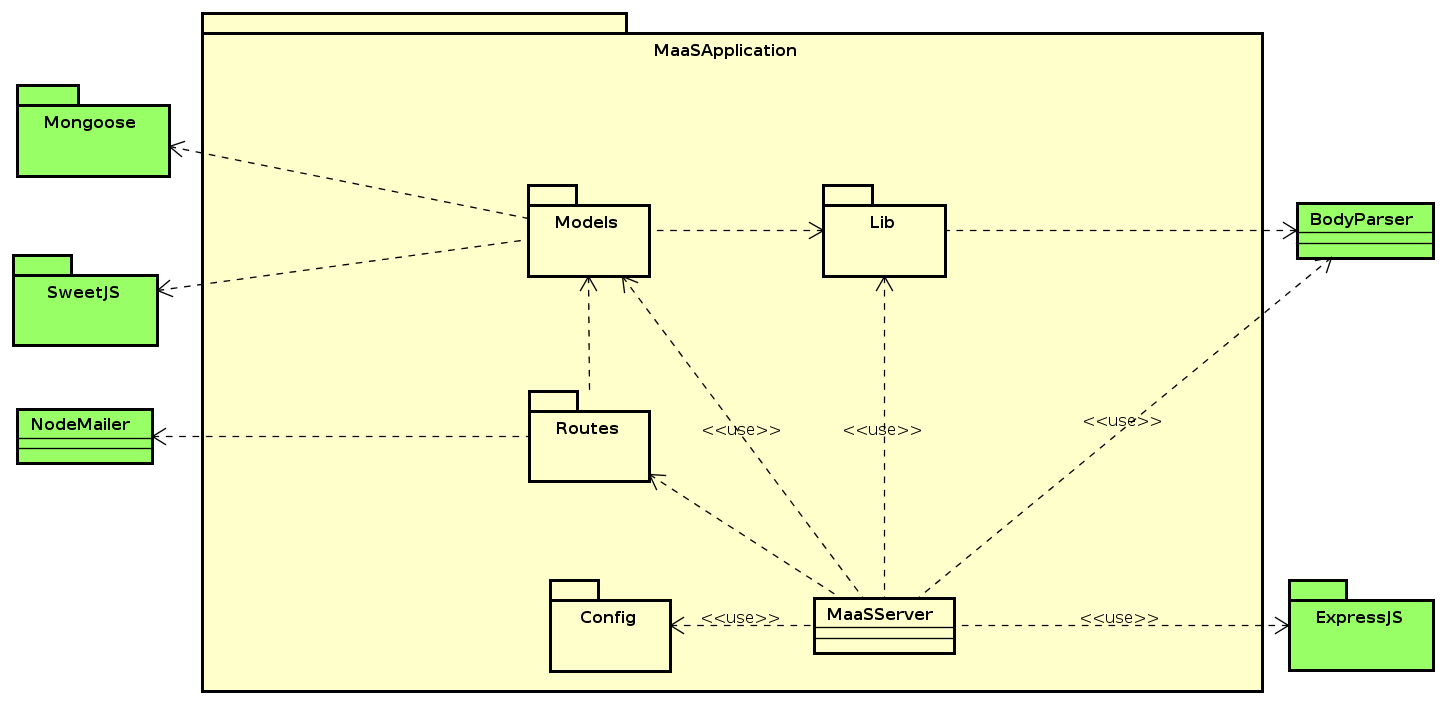
\includegraphics[width=0.8\textwidth]{res/sections/backend/generale.png}
\caption{Diagramma dei package}
\end{figure}

\subsubsection{Package MaaSApplication}
\paragraph*{Descrizione}
Package che racchiude tutta l'applicazione MaaS.

\paragraph*{Package contenuti}
\begin{itemize}
\item Models
\item Routes
\item Config
\item Lib
\end{itemize}

\paragraph*{Moduli contenuti}
\begin{itemize}
\item MaaSServer
\end{itemize}

\begin{figure}[H]
\centering
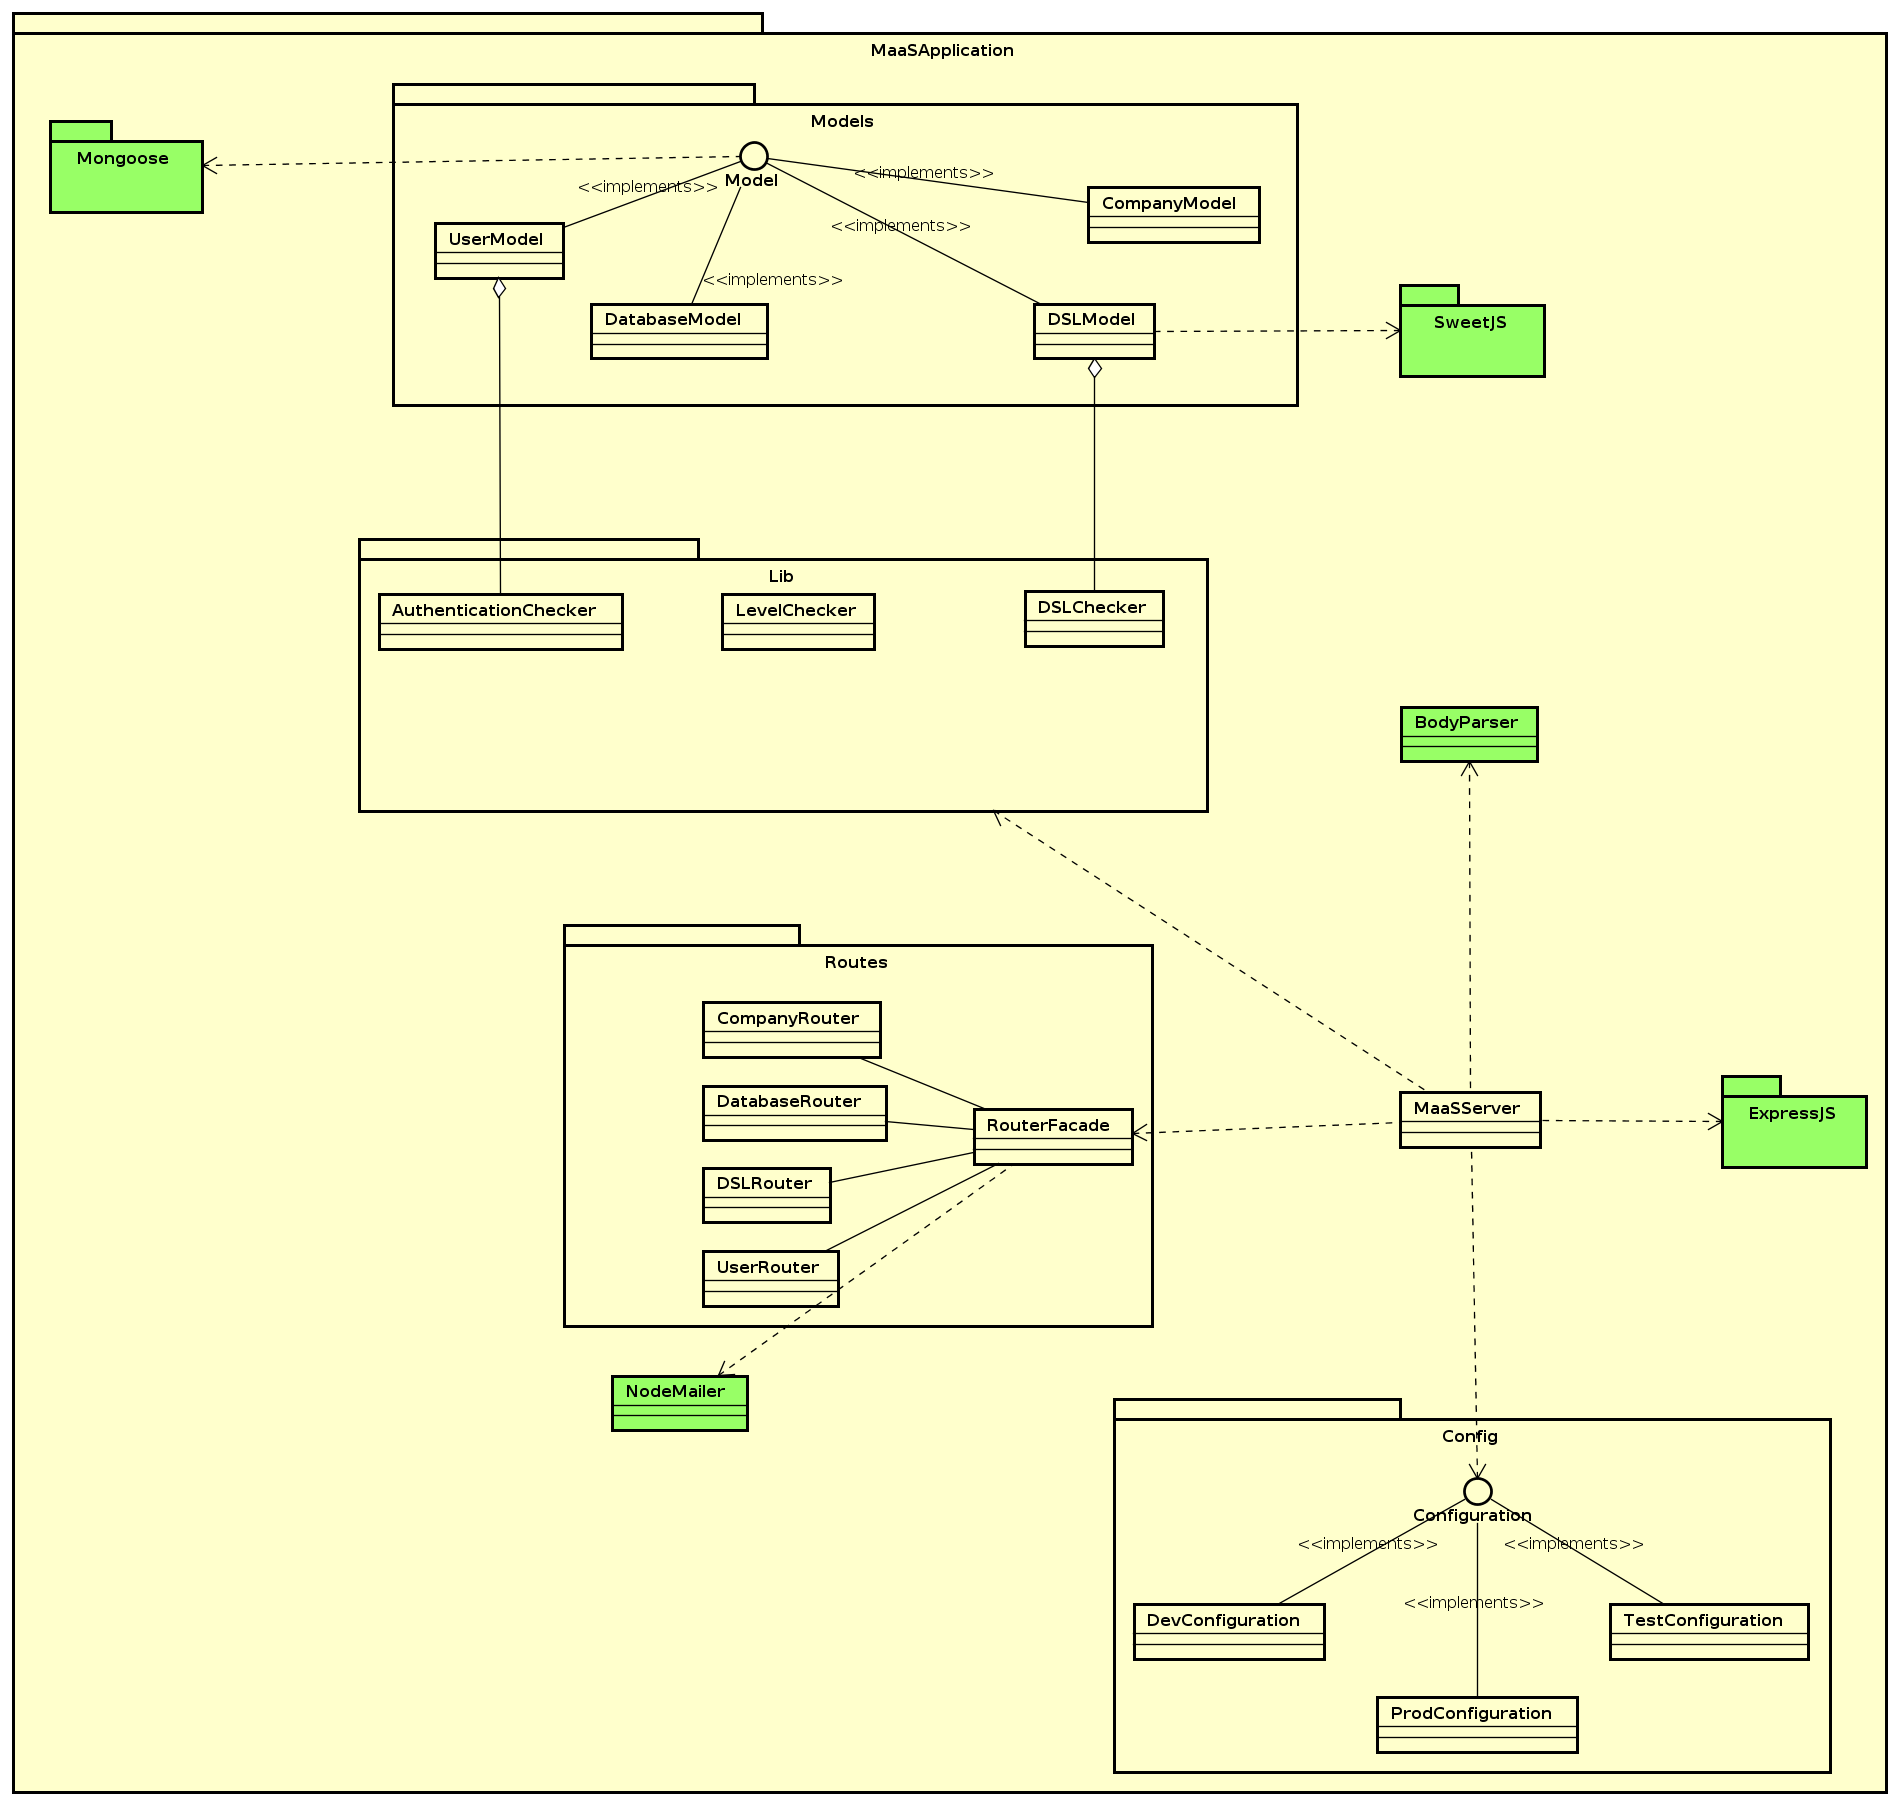
\includegraphics[width=0.8\textwidth]{res/sections/backend/collegamenti.png}
\caption{Diagramma dei package completo dei componenti per ciascun package}
\end{figure}

\subsubsection{Package Models}
\paragraph*{Descrizione}
Package che racchiude i moduli contenenti la business logic dell'applicazione. Ciascuno di questi moduli implementa un modello Mongoose e definisce i metodi con cui interagirvi (aggiungere, rimuovere e modificare i contenuti). \\
Rappresenta la parte M (Model) del design pattern MVC.

\paragraph*{Moduli contenuti}
\begin{itemize}
\item UserModel
\item DSLModel
\item CompanyModel
\item DatabaseModel
\end{itemize}

\paragraph*{Interfacce contenute}
\begin{itemize}
\item Model
\end{itemize}

\begin{figure}[H]
\centering
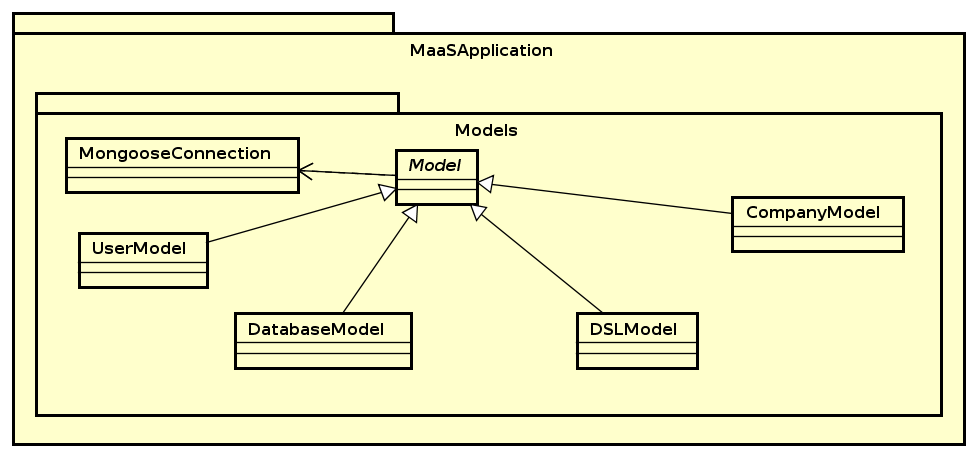
\includegraphics[width=0.8\textwidth]{res/sections/backend/models.png}
\caption{Diagramma delle classi del package Models}
\end{figure}

\paragraph{UserModel}
\paragraph*{Descrizione}

Racchiude la business logic legata agli utenti. Viene implementato tramite Module pattern di Javascript. 

\paragraph*{Utilizzo}
Il modello viene utilizzato sia per la rappresentazione di un utente nell'applicazione, sia per l'autenticazione nel sistema.

\paragraph*{Relazioni con altri moduli}
\begin{itemize}
\item Mongoose
\item Mongoose-validator
\item AuthenticationChecker
\end{itemize}

\paragraph{CompanyModel}
\paragraph*{Descrizione}

Racchiude la business logic legata alle Company. Viene implementato tramite Module pattern di Javascript. 

\paragraph*{Utilizzo}
Il modello rappresenta una Company nel sistema.

\paragraph*{Relazioni con altri moduli}
\begin{itemize}
\item Mongoose
\item Mongoose-validator
\end{itemize}

\paragraph{DatabaseModel}
\paragraph*{Descrizione}

Racchiude la business logic legata al collegamento con i database delle Company. Viene implementato tramite Module pattern di Javascript. 

\paragraph*{Utilizzo}
Il modello rappresenta la connessione ad un database aziendale di una company. Contiene i dati per effettuare l'accesso al database e il riferimento alle collections definite su tale database, permettendo così all'utente di poter definire per ciascuna collection la possibilità di interagirvi da parte di tutti i membri della propria Company o solo degli admin.

\paragraph*{Relazioni con altri moduli}
\begin{itemize}
\item Mongoose
\item Mongoose-validator
\end{itemize}

\paragraph{DSLModel}
\paragraph*{Descrizione}

Racchiude la business logic legata alle specifiche DSL. Viene implementato tramite Module pattern di Javascript. 

\paragraph*{Utilizzo}
Il modello viene utilizzato per la rappresentazione delle specifiche DSL. Contiene i dati di tali specifiche e le funzioni per poter estrarre i dati richiesti da una specifica DSL.

\paragraph*{Relazioni con altri moduli}
\begin{itemize}
\item Mongoose
\item Mongoose-validator
\item DSLChecker
\item DatabaseModel
\end{itemize}

\paragraph{Model}
\paragraph*{Descrizione}
Interfaccia comune a tutti i modelli usati da MaaS.

\paragraph*{Utilizzo}
Viene utilizzata come base per UserModel, CompanyModel, DSLModel e DatabaseModel.

\paragraph*{Relazione con altri moduli}
\begin{itemize}
\item Mongoose
\item UserModel
\item CompanyModel
\item DSLModel
\item DatabaseModel
\end{itemize}

\subsubsection{Package Routes}
\paragraph*{Descrizione}
Il package Routes contiene l'implementazione dei Router definiti da ExpressJS. Il package è costituito da una serie di moduli che implementano gli endpoint per le API.
I moduli vengono suddivisi in base al modello che utilizzano. Ciascuna route definita inoltre ha il compito di richiamare i middleware necessari.
La definizione delle API seguirà la descrizione riportata nella sezione apposita di questo documento.\\
Reppresenta la parte C (Controller) del design pattern MVC.

\paragraph*{Moduli contenuti}
\begin{itemize}
\item UserRouter
\item CompanyRouter
\item DSLRouter
\item DatabaseRouter
\item RouterFacade
\end{itemize}

\paragraph*{Interfacce contenute}
\begin{itemize}
\item Router
\end{itemize}

\begin{figure}[H]
\centering
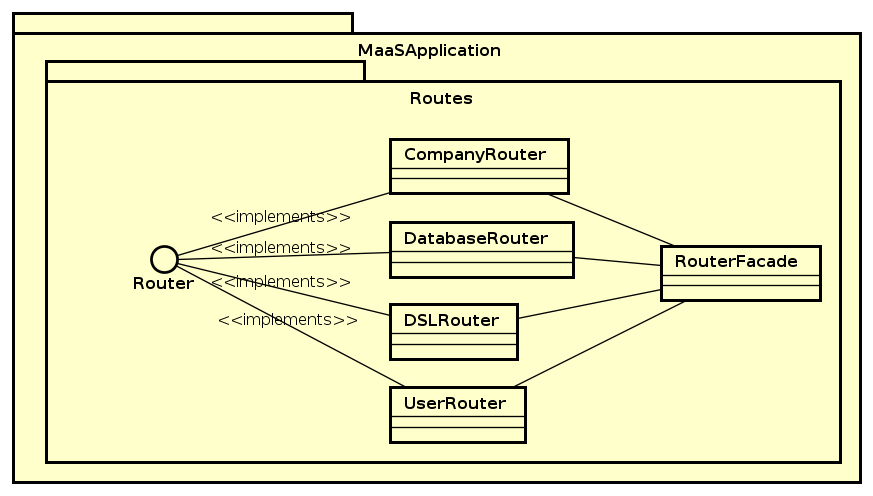
\includegraphics[width=0.8\textwidth]{res/sections/backend/routes.png}
\caption{Diagramma delle classi del package Routes}
\end{figure}

\paragraph{UserRouter}
\paragraph*{Descrizione}
Questo modulo contiene la definizione degli endpoint riguardanti gli utenti. 

\paragraph*{Relazione con altri moduli}
\begin{itemize}
\item AuthenticationChecker
\item UserModel
\end{itemize}

\paragraph{CompanyRouter}
\paragraph*{Descrizione}
Questo modulo contiene la definizione degli endpoint riguardanti le company.

\paragraph*{Relazione con altri moduli}
\begin{itemize}
\item AuthenticationChecker
\item CompanyModel
\end{itemize}

\paragraph{DSLRouter}
\paragraph*{Descrizione}
Questo modulo contiene la definizione degli endpoint riguardanti le specifiche DSL.

\paragraph*{Relazione con altri moduli}
\begin{itemize}
\item AuthenticationChecker
\item DSLModel
\end{itemize}

\paragraph{DatabaseRouter}
\paragraph*{Descrizione}
Questo modulo contiene la definizione degli endpoint riguardanti le connessioni ai database aziendali.

\paragraph*{Relazione con altri moduli}
\begin{itemize}
\item AuthenticationChecker
\item DatabaseModel
\end{itemize}

\paragraph{RouterFacade}
\paragraph*{Descrizione}
Oggetto che implementa il Facade Design Pattern. Tale oggetto incorpora tutti gli endpoint definiti dagli altri router.

\paragraph*{Relazione con altri moduli}
\begin{itemize}
\item AuthenticationChecker
\item UserRouter
\item CompanyRouter
\item DSLRouter
\item DatabaseRouter
\end{itemize}

\paragraph{Router}
\paragraph*{Descrizione}
Interfaccia comune ai router usati da MaaS.

\paragraph*{Utilizzo}
Viene utilizzata come base per UserRouter, CompanyRouter, DSLRouter e DatabaseRouter.

\paragraph*{Relazione con altri moduli}
\begin{itemize}
\item BodyParser
\item UserRouter
\item CompanyRouter
\item DSLRouter
\item DatabaseRouter
\end{itemize}

\subsubsection{Package Config}
\paragraph*{Descrizione}
Questo package contiene la classe Configuration che, in base alla variabile d'ambiente NODE\_ENV, restituisce l'oggetto contenente tutte le informazioni utili alla configurazione del server.

\paragraph*{Moduli contenuti}
\begin{itemize}
\item Configuration
\item DevConfiguration
\item TestConfiguration
\item ProdConfiguration
\end{itemize}

\paragraph*{Interfacce contenute}
\begin{itemize}
\item Configuration
\end{itemize}

\begin{figure}[H]
\centering
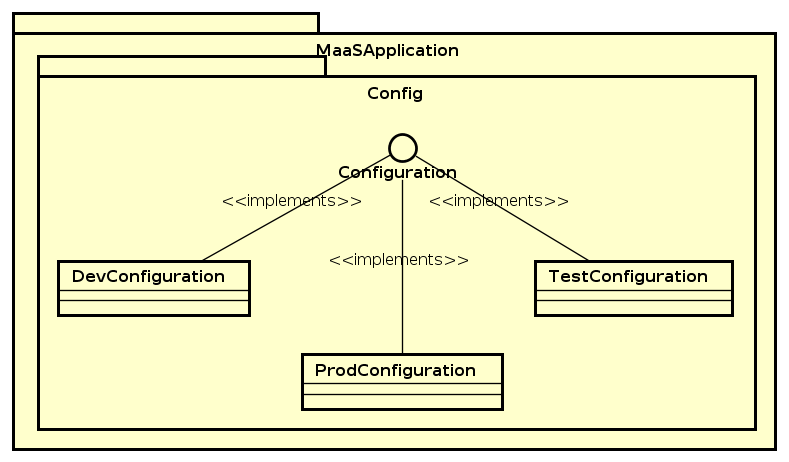
\includegraphics[width=0.8\textwidth]{res/sections/backend/config.png}
\caption{Diagramma delle classi del package Config}
\end{figure}

\paragraph{DevConfiguration}
\paragraph*{Descrizione}
Configurazione usata durante lo sviluppo.

\paragraph*{Utilizzo}
Viene utilizzata per configurare l'ambiente di lavoro durante lo sviluppo di MaaS.

\paragraph{TestConfiguration}
\paragraph*{Descrizione}
Configurazione usata durante il test.

\paragraph*{Utilizzo}
Viene utilizzata per configurare l'ambiente di lavoro durante il test di MaaS.

\paragraph{ProdConfiguration}
\paragraph*{Descrizione}
Configurazione usata per il rilascio.

\paragraph*{Utilizzo}
Viene utilizzata per configurare l'ambiente di lavoro per la consegna di MaaS.

\paragraph{Configuration}
\paragraph*{Descrizione}
Interfaccia comune alle configurazioni usate da MaaS.

\paragraph*{Utilizzo}
Viene utilizzata come base per DevConfiguration, TestConfiguration e ProdConfiguration.

\paragraph*{Relazione con altri moduli}
\begin{itemize}
\item MaaSServer
\end{itemize}

\subsubsection{Package Lib}
\paragraph*{Descrizione}
Questo package contiene tutti i moduli di supporto al sistema e i middlewares generici per ExpressJS.

\paragraph*{Moduli contenuti}
\begin{itemize}
\item LevelChecker
\item AuthenticationChecker
\item DSLChecker
\end{itemize}

\paragraph{Interfacce contenute}
\begin{itemize}
\item Middleware
\end{itemize}

\begin{figure}[H]
\centering
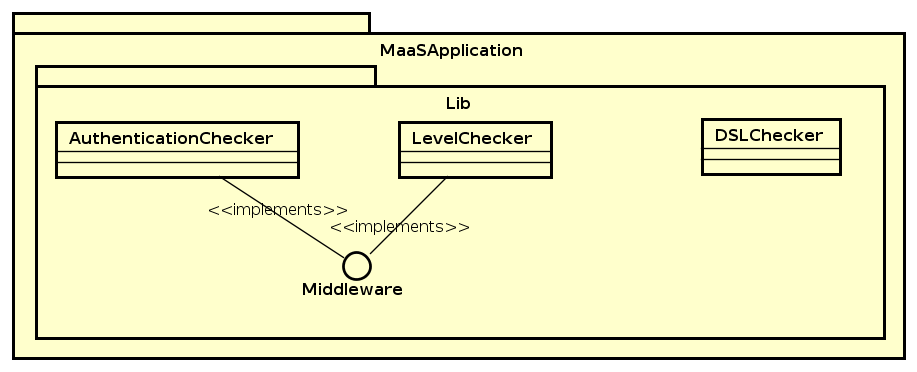
\includegraphics[width=0.8\textwidth]{res/sections/backend/lib.png}
\caption{Diagramma delle classi del package Lib}
\end{figure}

\paragraph{LevelChecker}
\paragraph*{Descrizione}
Middleware che si occupa di verificare se l'utente che effettua una richiesta al server ha i livelli minimi di accesso per poterla eseguire.

\paragraph*{Utilizzo}
Viene utilizzato nelle routes in cui deve essere garantito un livello utente minimo di accesso per portare a termine la richiesta.

\paragraph*{Relazione con altri moduli}
\begin{itemize}
\item Router
\end{itemize}

\paragraph{AuthenticationChecker}
\paragraph*{Descrizione}
Modulo che definisce due middleware: uno per effettuare il login, l'altro per l'autenticazione di una richiesta.

\paragraph*{Utilizzo}
Questo modulo viene utilizzato per definire l'endpoint per effettuare il login all'applicazione e offre il middleware che permette di autenticare le richieste. Tale middleware si occuperà di estrarre il token dalle richieste, verificarne la correttezza e aggiungere l'utente verificato nella richiesta per i prossimi middleware.

\paragraph*{Relazione con altri moduli}
\begin{itemize}
\item Router
\end{itemize}

\paragraph{DSLChecker}
\paragraph*{Descrizione}
Modulo che verifica la correttezza sintattica e di contenuto di una specifica DSL.

\paragraph*{Utilizzo}
Questo modulo viene richiamato in DSLModel per verificare che la specifica DSL che viene salvata o modificata sia valida per l'esecuzione.

\paragraph*{Relazione con altri moduli}
\begin{itemize}
\item DSLModel
\end{itemize}

\paragraph{Middleware}
\paragraph*{Descrizione}
Interfaccia comune ai middlware usati da MaaS.

\paragraph*{Utilizzo}
Viene utilizzata come base per AuthenticationChecker e per LevelChecker.

\paragraph*{Relazione con altri moduli}
\begin{itemize}
\item BodyParser
\item AuthenticationChecker
\item LevelChecker
\end{itemize}

\subsubsection{Modulo MaaSServer}
\paragraph*{Descrizione}
Modulo principale dell'applicazione.

\paragraph*{Utilizzo}
Viene 

\paragraph*{Relazione con altri moduli}
\begin{itemize}
\item Config
\item RouterFacade
\item BodyParser
\end{itemize}

\paragraph*{Relazione con altri package}
\begin{itemize}
\item Lib
\item ExpressJS
\end{itemize}

\subsubsection{Moduli integrati}
\paragraph{BodyParser}
\paragraph*{Descrizione}
?????????????????

\paragraph*{Utilizzo}
??????????????????

\paragraph{NodeMailer}
\paragraph*{Descrizione}
Permette di inviare delle email.

\paragraph*{Utilizzo}
È usato per inviare email agli utenti di MaaS.

\subsubsection{Framework integrati}
\paragraph{SweetJS}
\paragraph*{Descrizione}
?????????????????

\paragraph*{Utilizzo}
??????????????????

\paragraph{ExpressJS}
\paragraph*{Descrizione}
Framework per la creazione e la gestione di API REST.

\paragraph*{Utilizzo}
Utilizzato come base per la struttura del server.

\paragraph{Mongoose}
\paragraph*{Descrizione}
Framework per interfacciarsi con MongoDB.

\paragraph*{Utilizzo}
Utilizzato per la gestione dei dati su database MongoDB.


%-----------------------------------------------
\subsubsection{Comunicazione tra client e server}
\huge{LO TENIAMO????}\\
Per la creazione del back end di MaaS si è deciso di utilizzare Node.js e, in particolare, il framework ExpressJS, che permette la creazione semplificata di server REST. Il lato back end sarà quindi costituito da un insieme di API protette da strati diversi di sicurezza. \\
Ciascuna API del webserver fornirà una risposta in formato JSON per permettere la fruizione delle informazioni. Fornirà nello stesso formato anche gli eventuali messaggi di errore generati nel corpo dei metodi del server. Tali messaggi di errore saranno così composti: 
\begin{verbatim}
{
    "code":     [Codice definito nel protocollo HTTP, che identifica univocamente
                 la tipologia del problema]
    "message":  [Messaggio che definisce in dettaglio la tipologia dell'errore]
    ["data":   [Opzionale, trasporta i dati in cui si è verificato l'errore]]
}
\end{verbatim}
I codici di errore saranno del tipo 4xx (client error, la richiesta è sintatticamente scorretta o non può essere soddisfatta) o 5xx (server error, il server ha fallito nel soddisfare una richiesta apparentemente valida).
\subsubsection{Sicurezza}
Gli accessi alle API avranno 2 livelli di sicurezza. \\
Il primo livello è rappresentato dall'autenticazione: un utente non autenticato riceverà un errore se richiede una API protetta. Verrà implementato con l'utilizzo di PassportJS, un middleware per ExpressJS che permette l'autenticazione di utenti nel sistema. In particolare verrà utilizzata la strategia passport-local per l'accesso al server, cioè le credenziali dell'utente risiederanno nel database locale. \\
Il secondo livello è definito in base al ruolo di appartenenza di un utente. Si occuperà di controllare i permessi assegnati ad un utente autenticato e di verificare la possibilità che possa o meno interagire con la risorsa richiesta. \\
I ruoli utente ammessi nell'applicazione sono: 
\begin{itemize}
\item \textbf{GUEST};
\item \textbf{MEMBER};
\item \textbf{ADMIN};
\item \textbf{OWNER};
\item \textbf{SUPERADMIN}.
\end{itemize}
Per il ruolo di SUPERADMIN è abilititato un set di API per la gestione dell'intera applicazione. Tali API non sono accessibili agli utenti con altri ruoli.